\documentclass[11pt]{article}

\usepackage{../theory}


\begin{document}
\date{}
%\date{Feb 3, 2020}

\coverpage{4}

\newpage
\section*{Problem 1}

Let ${\cal B}$ be the set of all infinite sequences over $\{a,b\}$. Show that
${\cal B}$ is uncountable, using a proof by diagonalization. \\

\noindent
{\bf Proof: } We prove that ${\cal B}$ is uncountable by contradiction, that is, we assume that ${\cal B}$ is countable. Since ${\cal B}$ is countable, we know there exists a bijective map \\ 
$f: {\cal B} \longrightarrow {\cal N}$. We now construct an element $b \in {\cal B}$ that violates the surjective property of $f$, that is, there exists no $n \in {\cal N}$ such that $f(n) = b$. \parspace
For $i \in {\cal N}$, let $f(i) = a$. We then choose $b_i \neq a_i$ (where $*_i$ means the $i^{th}$ element of $*$). To be explicit, if $a_i = a$, then $b_i = b$. Alternatively, if $a_i = b$, then $b_i = a$. \parspace
We have now constructed $b \in {\cal B}$ (the Codomain) such that there exists no $n \in {\cal N}$ (the Domain) where $f(n) = b$. This means that the map $f$ is no longer surjective. Thus, in assuming that ${\cal B}$ is countable, we have encountered a contradiction. So it must be the case that ${\cal B}$ is uncountable.

$\hfill \Box$
\newpage

\section*{Problem 2}

Let $T=\{ (i,j,k) \mid i,j,k \in {\cal N} \}$. Show that $T$ is countable. \\

\noindent
{\bf Proof: } To show that $T$ is countable, we must that there exists a bijection $f : {\cal N} \longrightarrow T$. \parspace
To show this, we first present a more general lemma: for $U$ and $V$, two countably infinite sets, the cartesian product $U \times V$ is countable. \parspace
Since both $U$ and $V$ are countably infinite, there exists two bijective maps \\
$u: {\cal N} \longrightarrow U$ and $v: {\cal N} \longrightarrow V$ and all the elements of $U \times V$ can be listed as
\begin{center}
	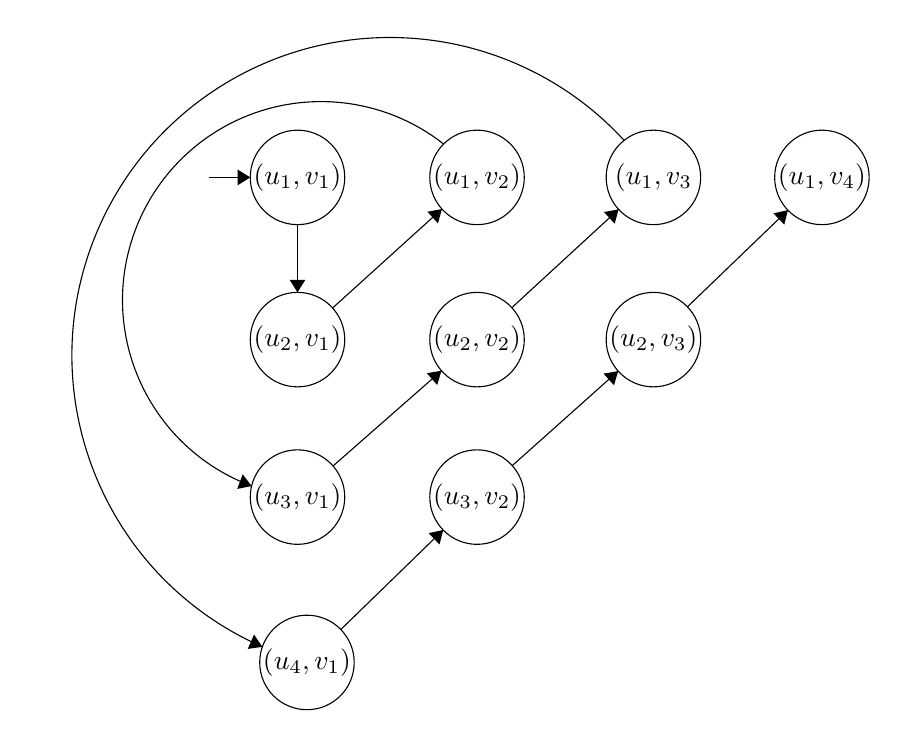
\begin{tikzpicture}[scale=0.2]
	\tikzstyle{every node}+=[inner sep=0pt]
	\draw [black] (21.1,-13.5) circle (3);
	\draw (21.1,-13.5) node {$(u_1,v_1)$};
	\draw [black] (32.5,-13.5) circle (3);
	\draw (32.5,-13.5) node {$(u_1,v_2)$};
	\draw [black] (43.7,-13.5) circle (3);
	\draw (43.7,-13.5) node {$(u_1,v_3$};
	\draw [black] (21.1,-23.8) circle (3);
	\draw (21.1,-23.8) node {$(u_2,v_1)$};
	\draw [black] (32.5,-23.8) circle (3);
	\draw (32.5,-23.8) node {$(u_2,v_2)$};
	\draw [black] (43.7,-23.8) circle (3);
	\draw (43.7,-23.8) node {$(u_2,v_3)$};
	\draw [black] (21.1,-33.8) circle (3);
	\draw (21.1,-33.8) node {$(u_3,v_1)$};
	\draw [black] (32.5,-33.8) circle (3);
	\draw (32.5,-33.8) node {$(u_3,v_2)$};
	\draw [black] (21.7,-44.3) circle (3);
	\draw (21.7,-44.3) node {$(u_4,v_1)$};
	\draw [black] (54.4,-13.5) circle (3);
	\draw (54.4,-13.5) node {$(u_1,v_4)$};
	\draw [black] (15.5,-13.5) -- (18.1,-13.5);
	\fill [black] (18.1,-13.5) -- (17.3,-13) -- (17.3,-14);
	\draw [black] (21.1,-16.5) -- (21.1,-20.8);
	\fill [black] (21.1,-20.8) -- (21.6,-20) -- (20.6,-20);
	\draw [black] (23.33,-21.79) -- (30.27,-15.51);
	\fill [black] (30.27,-15.51) -- (29.35,-15.68) -- (30.02,-16.42);
	\draw [black] (18.191,-33.095) arc (-110.43689:-308.19818:12.602);
	\fill [black] (18.19,-33.1) -- (17.62,-32.35) -- (17.27,-33.28);
	\draw [black] (23.36,-31.82) -- (30.24,-25.78);
	\fill [black] (30.24,-25.78) -- (29.31,-25.93) -- (29.97,-26.68);
	\draw [black] (34.71,-21.77) -- (41.49,-15.53);
	\fill [black] (41.49,-15.53) -- (40.56,-15.7) -- (41.24,-16.44);
	\draw [black] (18.873,-43.305) arc (-113.64063:-317.43473:20.193);
	\fill [black] (18.87,-43.31) -- (18.34,-42.53) -- (17.94,-43.44);
	\draw [black] (23.85,-42.21) -- (30.35,-35.89);
	\fill [black] (30.35,-35.89) -- (29.43,-36.09) -- (30.12,-36.81);
	\draw [black] (34.74,-31.8) -- (41.46,-25.8);
	\fill [black] (41.46,-25.8) -- (40.53,-25.96) -- (41.2,-26.7);
	\draw [black] (45.86,-21.72) -- (52.24,-15.58);
	\fill [black] (52.24,-15.58) -- (51.32,-15.78) -- (52.01,-16.5);
	\end{tikzpicture}
\end{center}
In the same way that we showed that the set of rational numbers is countable, we can also show that $U \times V$ is also countable. So the lemma is shown to be true. \parspace
Using this lemma, we now show that $T$ is countable. To do this, we first note that $T = {\cal N} \times {\cal N} \times {\cal N}$. Let ${\cal M} = {\cal N} \times {\cal N}$, then ${\cal M}$ is certainly countable (by the above lemma) since ${\cal M}$ is the product of two countable infinite sets. Additionally, $T = {\cal M} \times {\cal N}$. We can then apply the lemma again to say that $T$ must also be countably infinite. A countably infinite set is countable so $T$ is countable.

$\hfill \Box$
\newpage

\section*{Problem 3}

Let $INFINITE_{PDA}=\{ \langle M \rangle |M$ is a PDA and $L(M)$ is an infinite language$\}$.
Show that $INFINITE_{PDA}$ is decidable.
\newline

\noindent
{\bf Proof: } We show that $INFINITE_{PDA}$ is decidable by giving a Turing Machine that decides it. Before doing so, we give some background knowledge. \parspace
By the pumping lemma, all infinite Context Free Languages have a derivation have a sufficiently long string $s = uvxyz$ such that $uv^i xy^i z$ remains in the language for all $i \geq 0$. So there must exist a derivation step for $s$ that looks like $V \derives uVx$. Also recall that the pumping length (the minimum length for $s$) is finite. Now consider the TM A. \parspace
$A = $ ``On input P a PDA: \\
\indent \textbf{1. } Convert P to an equivalent CFG G in Chomsky Normal Form\\
\indent \textbf{2. } Repeat for each natural number (referenced as $n$) \\
\indent \textbf{3. } \indent Compute all derivations of $G$ with length $n$ \\
\indent \textbf{4. } \indent If there are no derivations of length $n$, \textit{reject} \\
\indent \textbf{5. } \indent If there is a derivation step of the form $V \derives uVx$, \textit{accept}'' \parspace
We know that $A$ will terminate since a finite CFL will have a finite number of derivations and all infinite CFL satisfy the pumping lemma. So, one of steps \textbf{4} and \textbf{5} must be true for some $n$. So $A$ decides $INFINITE_{PDA}$.

$\hfill \Box$
\newpage

\section*{Problem 4}

Let $\Sigma=\{a,b\}$. Define the following language {\em ODD}$_{TM}$: \\
{\em ODD}$_{TM}=\{ \langle M \rangle \mid M$ is a TM and $L(M)$ contains only strings of odd length $\}$.

Prove that {\em ODD}$_{TM}$ is undecidable. \\

\noindent
{\bf Proof: } As is typical in proving undecidability, we use reduction in this proof. For the sake of contradiction, we assume that a $TM$ $R$ decides {\em ODD}$_{TM}$. Now consider the following Turing Machine (where $M$ and $w$ reference $< M, w >$ from $A_{TM}$). \parspace
$M_1 = $ ``On input x: \\
	\indent \textbf{1. } If $|x|$ is odd, \textit{accept} \\
	\indent \textbf{2. } If $|x|$ is even, run $M$ on $w$ and \textit{accept} if $M$ accepts $w$'' \parspace
Then $L(M_1)$ will always contain at least all strings of odd length. However, $L(M_1)$ will only contain strings of even length if $M$ accepts $w$. That is, the membership of $M_1$ in $ODD_{TM}$ depends entirely on whether $M$ accepts $w$. We will now construct a $TM$ to decide $A_{TM}$: \parspace
$S = $ ``On input $\langle M, w \rangle $: \\
	\indent \textbf{1. } Construct $M_1$ as above \\
	\indent \textbf{2. } Run $R$ on input $\langle M_1 \rangle $ \\
	\indent \textbf{3. } If $R$ accepts, \textit{reject} \\
	\indent \textbf{4. } If $R$ rejects, \textit{accept}'' \parspace
So in assuming that $R$ (a decider for {\em ODD}$_{TM}$) existed, we found that we could decide $A_{TM}$. Yet, this cannot be the case since we know $A_{TM}$ to be undecidable. Therefore, no such $R$ can exist and {\em ODD}$_{TM}$ must be undecidable as well.

$\hfill \Box$
\newpage

\section*{Problem 5}

Show that $EQ_{CFG}$ is undecidable.
\newline

\noindent
{\bf Proof: } First note that \\\\
\indent $EQ_{CFG} := \{ \langle G_1, G_2 \rangle \mid G_1$ and $G_2$ are CFGs and $L(G_1) = L(G_2) \}$ \parspace
Now recall from Theorem 5.13 that $ALL_{CFG} := \{ \langle G \rangle \mid G $ is a CFG and $L(G) = \Sigma ^* \} $ is undecidable. Now, for the sake of contradiction, we assume that $EQ_{CFG}$ is decidable by a TM $R$. Let us now give a TM $S$ that decides $ALL_{CFG}$. \parspace
$S = $ ``On input $\langle G \rangle $ a CFG: \\
\indent \textbf{1. } Let $H$ be a CFG where $L(H) = \Sigma ^*$ \\
\indent \textbf{2. } Run TM $R$ on input $\langle H, G \rangle $ \\
\indent \textbf{3. } If $R$ accepts, \textit{accept}. If $R$ rejects, \textit{reject}. \parspace
Under the assumption that a TM $R$ that decides $EQ_{CFG}$ existed, we were able to show that $ALL_{CFG}$ was decidable. However, we know $ALL_{CFG}$ to be undecidable so we have reached a contradiction. Thus, $EQ_{CFG}$ must be undecidable.

$\hfill \Box$
\newpage

\section*{Problem 6}

Show that $EQ_{CFG}$ is co-Turing-recognizable.
\newline

\noindent
{\bf Proof: } First recall that a language is co-Turing-recognizable if it is the complement of a Turing-recognizable language. Also recall that \\\\
\indent $EQ_{CFG} := \{ \langle G_1, G_2 \rangle \mid G_1$ and $G_2$ are CFGs and $L(G_1) = L(G_2) \}$ \parspace
So our task is then to show that $\overline{EQ}_{CFG}$ is Turing recognizable. But what is $\overline{EQ}_{CFG}$? It is shown below \\\\
\indent $\overline{EQ}_{CFG} = \{ \langle G_1, G_2 \rangle \mid G_1$ and $G_2$ are CFGs and $L(G_1) \neq L(G_2)$. \parspace
Now note that the alphabet $\Sigma ^*$ is countably infinite (there is a correspondence between the natural numbers and $\Sigma ^*$). Also note that $A_{CFG}$ (from Theorem 4.7) decides whether a given CFG accepts a given string. With this in mind, we now give a Turing machine that recognizes $\overline{EQ}_{CFG}$. Consider the following Turing Machine A. \parspace
A = ``On input $G_1$ and $G_2$ (both Context Free Grammars): \\
\indent \textbf{1. } Repeat the steps below \\
\indent \textbf{2. } \indent Take $w$, the next member of $\Sigma ^*$ and compute $A_{CFG}$ for $\langle G_1, w \rangle $ and \indent \indent \indent $\langle G_2, w \rangle $ \\
\indent \textbf{3. } \indent If above results differ, \textit{accept}'' \parspace
The TM A recognizes $\overline{EQ}_{CFG}$, so $EQ_{CFG}$ is co-Turing-recognizable.

$\hfill \Box$
\newpage

\section*{Problem 7}

Find a match in the following instance of the Post Correspondence Problem.
$$  \left\{
	\left[ \dfrac{ab}{abab} \right], 
	\left[ \dfrac{b}{a} \right], 
	\left[ \dfrac{aba}{b} \right],
	\left[ \dfrac{aa}{a} \right] \right\} $$
\newline

\noindent
{\bf Proof: } A match in the Post Correspondence Problem is a list of dominos (allowing repetitions) such that reading the top gives the same result as reading the bottom. With this definition, the following is a match
$$  \left[ \dfrac{aa}{a} \right]
	\left[ \dfrac{aa}{a} \right]
	\left[ \dfrac{b}{a} \right]
	\left[ \dfrac{ab}{abab} \right] = \dfrac{aaaabab}{aaaabab} $$

$\hfill \Box$
\newpage

\end{document}
